% !TEX root = ../main.tex
\chapter{Ultrashort-Pulse Intuition}
\label{app:phase_kick_intuition}

This appendix collects an optional geometric intuition for the role of pulse carrier phases in pathway selection. It complements the formal treatment in~\autoref{subsec:phase_matching_condition,subsec:rephasing_nonrephasing,sec:phase_cycling} without changing the main derivation used in the thesis.

\section{Carrier Phase, Pulse Area, and Bloch-Sphere Picture}
\label{app:sec:phase_kick_pulse_area_intuition}

The carrier phases $\phi_j$ in~\autoref{eq:E_three_pulses_space} are experimentally controlled parameters that imprint well-defined phase factors on driven coherences and hence on the nonlinear polarisation. This provides the pathway selection used throughout this thesis.
This geometric picture is used as intuition. All quantitative results in this thesis are obtained from the full, numerically exact propagation and the phase-selection procedures developed in~\autoref{sec:phase_cycling}.

A visual interpretation arises for a resonantly driven two-level system within the RWA, where $\phi_j$ sets the rotation axis of the drive.
Writing the complex Rabi frequency of pulse $j$ as
\begin{equation}
    \Omega_j(t) \equiv \boldsymbol{\mu}_{eg}\cdot\boldsymbol{E}_j(t),
\end{equation}
the interaction Hamiltonian in the laser-rotating frame can be expressed as
\begin{equation}
    \hat{H}_{\mathrm{int},j}(t)
    \;\propto\;
    \Omega_j(t-t_j)
\Big( e^{-\mathrm{i}\phi_j}\,\ket{e}\!\bra{g} + e^{+\mathrm{i}\phi_j}\,\ket{g}\!\bra{e} \Big).
    \label{eq:Hint_phasekick}
\end{equation}
Changing $\phi_j$ rotates the complex drive while leaving the pulse envelope unchanged. On the Bloch sphere this corresponds to a rotation about an equatorial axis with azimuth angle $\phi_j$ (cf.~\cite{grolletal2025fundamentalsheterodynewave}).

The pulse area
\begin{equation}
    \theta_j \;\equiv\; \int_{-\infty}^{\infty}\!\mathrm{d}t\,\Omega_j(t-t_j)
    \label{eq:pulse_area_def}
\end{equation}
sets the corresponding rotation angle.
In the idealised delta-pulse limit one replaces $\Omega_j(t-t_j)\to \theta_j\,\delta(t-t_j)$, so the pulse acts as an instantaneous unitary
\begin{equation}
    \hat{U}_j
    \;=\;
\exp\!\left[-\frac{\mathrm{i}\,\theta_j}{2}\,\big(\cos\phi_j\,\hat{\tau}_x+\sin\phi_j\,\hat{\tau}_y\big)\right],
    \label{eq:delta_pulse_unitary}
\end{equation}
where $\hat{\tau}_{x,y,z}$ denote the Pauli matrices.

\begin{figure}[htbp]
    \centering
    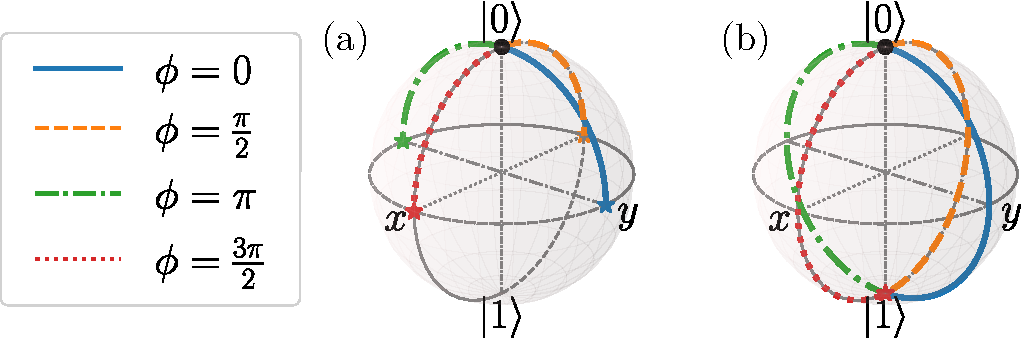
\includegraphics[width=0.7\textwidth]{figures/spctr_bloch_phase_rotation.pdf}
    \caption{Bloch-sphere visualization of one ultrashort interaction with a two-level system. The initial state is $\ket{0}$. Panels show examples for (a) $\theta=\pi/2$ and (b) $\theta=\pi$ with different carrier phase kicks $\phi$.}
    \label{fig:delta_phase_kick_bloch_rotation}
\end{figure}
